%%
%% Automatically generated file from DocOnce source
%% (https://github.com/doconce/doconce/)
%% doconce format latex program.do.txt --minted_latex_style=trac --latex_admon=paragraph --no_mako
%%
% #ifdef PTEX2TEX_EXPLANATION
%%
%% The file follows the ptex2tex extended LaTeX format, see
%% ptex2tex: https://code.google.com/p/ptex2tex/
%%
%% Run
%%      ptex2tex myfile
%% or
%%      doconce ptex2tex myfile
%%
%% to turn myfile.p.tex into an ordinary LaTeX file myfile.tex.
%% (The ptex2tex program: https://code.google.com/p/ptex2tex)
%% Many preprocess options can be added to ptex2tex or doconce ptex2tex
%%
%%      ptex2tex -DMINTED myfile
%%      doconce ptex2tex myfile envir=minted
%%
%% ptex2tex will typeset code environments according to a global or local
%% .ptex2tex.cfg configure file. doconce ptex2tex will typeset code
%% according to options on the command line (just type doconce ptex2tex to
%% see examples). If doconce ptex2tex has envir=minted, it enables the
%% minted style without needing -DMINTED.
% #endif

% #define PREAMBLE

% #ifdef PREAMBLE
%-------------------- begin preamble ----------------------

\documentclass[%
oneside,                 % oneside: electronic viewing, twoside: printing
final,                   % draft: marks overfull hboxes, figures with paths
10pt]{article}

\listfiles               %  print all files needed to compile this document

\usepackage{relsize,makeidx,color,setspace,amsmath,amsfonts,amssymb}
\usepackage[table]{xcolor}
\usepackage{bm,ltablex,microtype}

\usepackage[pdftex]{graphicx}

\usepackage[T1]{fontenc}
%\usepackage[latin1]{inputenc}
\usepackage{ucs}
\usepackage[utf8x]{inputenc}

\usepackage{lmodern}         % Latin Modern fonts derived from Computer Modern

% Hyperlinks in PDF:
\definecolor{linkcolor}{rgb}{0,0,0.4}
\usepackage{hyperref}
\hypersetup{
    breaklinks=true,
    colorlinks=true,
    linkcolor=linkcolor,
    urlcolor=linkcolor,
    citecolor=black,
    filecolor=black,
    %filecolor=blue,
    pdfmenubar=true,
    pdftoolbar=true,
    bookmarksdepth=3   % Uncomment (and tweak) for PDF bookmarks with more levels than the TOC
    }
%\hyperbaseurl{}   % hyperlinks are relative to this root

\setcounter{tocdepth}{2}  % levels in table of contents

% Tricks for having figures close to where they are defined:
% 1. define less restrictive rules for where to put figures
\setcounter{topnumber}{2}
\setcounter{bottomnumber}{2}
\setcounter{totalnumber}{4}
\renewcommand{\topfraction}{0.95}
\renewcommand{\bottomfraction}{0.95}
\renewcommand{\textfraction}{0}
\renewcommand{\floatpagefraction}{0.75}
% floatpagefraction must always be less than topfraction!
% 2. ensure all figures are flushed before next section
\usepackage[section]{placeins}
% 3. enable begin{figure}[H] (often leads to ugly pagebreaks)
%\usepackage{float}\restylefloat{figure}

\usepackage[framemethod=TikZ]{mdframed}

% --- begin definitions of admonition environments ---

% --- end of definitions of admonition environments ---

% prevent orhpans and widows
\clubpenalty = 10000
\widowpenalty = 10000

% --- end of standard preamble for documents ---


% insert custom LaTeX commands...

\raggedbottom
\makeindex
\usepackage[totoc]{idxlayout}   % for index in the toc
\usepackage[nottoc]{tocbibind}  % for references/bibliography in the toc

%-------------------- end preamble ----------------------

\begin{document}

% matching end for #ifdef PREAMBLE
% #endif

\newcommand{\exercisesection}[1]{\subsection*{#1}}


% ------------------- main content ----------------------



% ----------------- title -------------------------

\thispagestyle{empty}

\begin{center}
{\LARGE\bf
\begin{spacing}{1.25}
Master program in Computational Science  at the University of Oslo
\end{spacing}
}
\end{center}

% ----------------- author(s) -------------------------

\begin{center}
{\bf Tom Andersen${}^{1}$} \\ [0mm]
\end{center}


\begin{center}
{\bf Andreas Austeng${}^{2}$} \\ [0mm]
\end{center}


\begin{center}
{\bf Arne Bang Huseby${}^{3}$} \\ [0mm]
\end{center}


\begin{center}
{\bf John Burkart${}^{4}$} \\ [0mm]
\end{center}


\begin{center}
{\bf Michele Cascella${}^{5}$} \\ [0mm]
\end{center}


\begin{center}
{\bf Mats Carlsson${}^{6}$} \\ [0mm]
\end{center}


\begin{center}
{\bf Geir Dahl${}^{3}$} \\ [0mm]
\end{center}


\begin{center}
{\bf Simon Wolfgang Funke${}^{2, 7}$} \\ [0mm]
\end{center}


\begin{center}
{\bf Marianne Fyhn${}^{1}$} \\ [0mm]
\end{center}


\begin{center}
{\bf Viggo Hansteen${}^{6}$} \\ [0mm]
\end{center}


\begin{center}
{\bf Morten Hjorth-Jensen (chair)${}^{8}$} \\ [0mm]
\end{center}


\begin{center}
{\bf Joseph  Lacasce${}^{4}$} \\ [0mm]
\end{center}


\begin{center}
{\bf Katrine Langvad (admin)${}^{8}$} \\ [0mm]
\end{center}


\begin{center}
{\bf Anders Malthe-Sørenssen${}^{8}$} \\ [0mm]
\end{center}


\begin{center}
{\bf Kend-Andre Mardal${}^{3}$} \\ [0mm]
\end{center}


\begin{center}
{\bf Martin Reimers${}^{3}$} \\ [0mm]
\end{center}


\begin{center}
{\bf Knut Mørken${}^{3}$} \\ [0mm]
\end{center}


\begin{center}
{\bf Torbjørn Rognes${}^{2}$} \\ [0mm]
\end{center}


\begin{center}
{\bf Thomas Schuler${}^{4}$} \\ [0mm]
\end{center}


\begin{center}
{\bf Grete Stavik-Døvle (admin)${}^{8}$} \\ [0mm]
\end{center}


\begin{center}
{\bf Joakim Sundnes${}^{2, 7}$} \\ [0mm]
\end{center}

\begin{center}
% List of all institutions:
\centerline{{\small ${}^1$Department of Biosciences, University of Oslo}}
\centerline{{\small ${}^2$Department of Informatics, University of Oslo}}
\centerline{{\small ${}^3$Department of Mathematics, University of Oslo}}
\centerline{{\small ${}^4$Department of Geoscience, University of Oslo}}
\centerline{{\small ${}^5$Department of Chemistry, University of Oslo}}
\centerline{{\small ${}^6$Institute for Theoretical Astrophysics, University of Oslo}}
\centerline{{\small ${}^7$Simula Research Laboratory}}
\centerline{{\small ${}^8$Department of Physics, University of Oslo}}
\end{center}
    
% ----------------- end author(s) -------------------------


% --- begin date ---
\begin{center}
Planned start: Fall 2018
\end{center}
% --- end date ---

\vspace{1cm}


% !split
\subsection{Master program in Computational Science}

% --- begin paragraph admon ---
\paragraph{}
We propose a new Master of Science program at the Faculty of Mathematics and Natural Sciences of the University of Oslo. This program is called  \textbf{Computational Science}, with acronym  \textbf{CS}

The program is a collaboration between seven departments and classical disciplines:

\begin{itemize}
 \item Institute of Theoretical Astrophysics

 \item Department of Biosciences

 \item Department of Chemistry

 \item Department of Geoscience

 \item Department of Informatics

 \item Department of Mathematics

 \item Department of Physics
\end{itemize}

\noindent
The program will be administrated by the Department of Physics.

The program is multidisciplinary and all students who have completed
undergraduate studies in science and engineering, with a sufficient
quantitative background, are eligible.  The language of instruction is
Norwegian or English.
% --- end paragraph admon ---



% !split
\subsection{Strategic importance}

The program will educate the next generation of cross-disciplinary
science students with the knowledge, skills, and values needed to pose
and solve current and new scientific, technological and societal
challenges. The program will lay the foundation for cross-disciplinary
educational, research and innovation activities.

It is the first educational program to
comprehensively treat computation as the \emph{triple junction} of
algorithm development and analysis, high performance computing, and
applications to scientific and engineering modeling and data
science. This approach recognizes computation as a new discipline
rather than being decentralized into isolated sub-disciplines. The CS program
will  will enable application-driven computational modeling
while also exposing disciplinary computational scientists to
advanced tools and techniques, which will ignite new
transformational connections in research and education.

\vspace{6mm}

% inline figure
\centerline{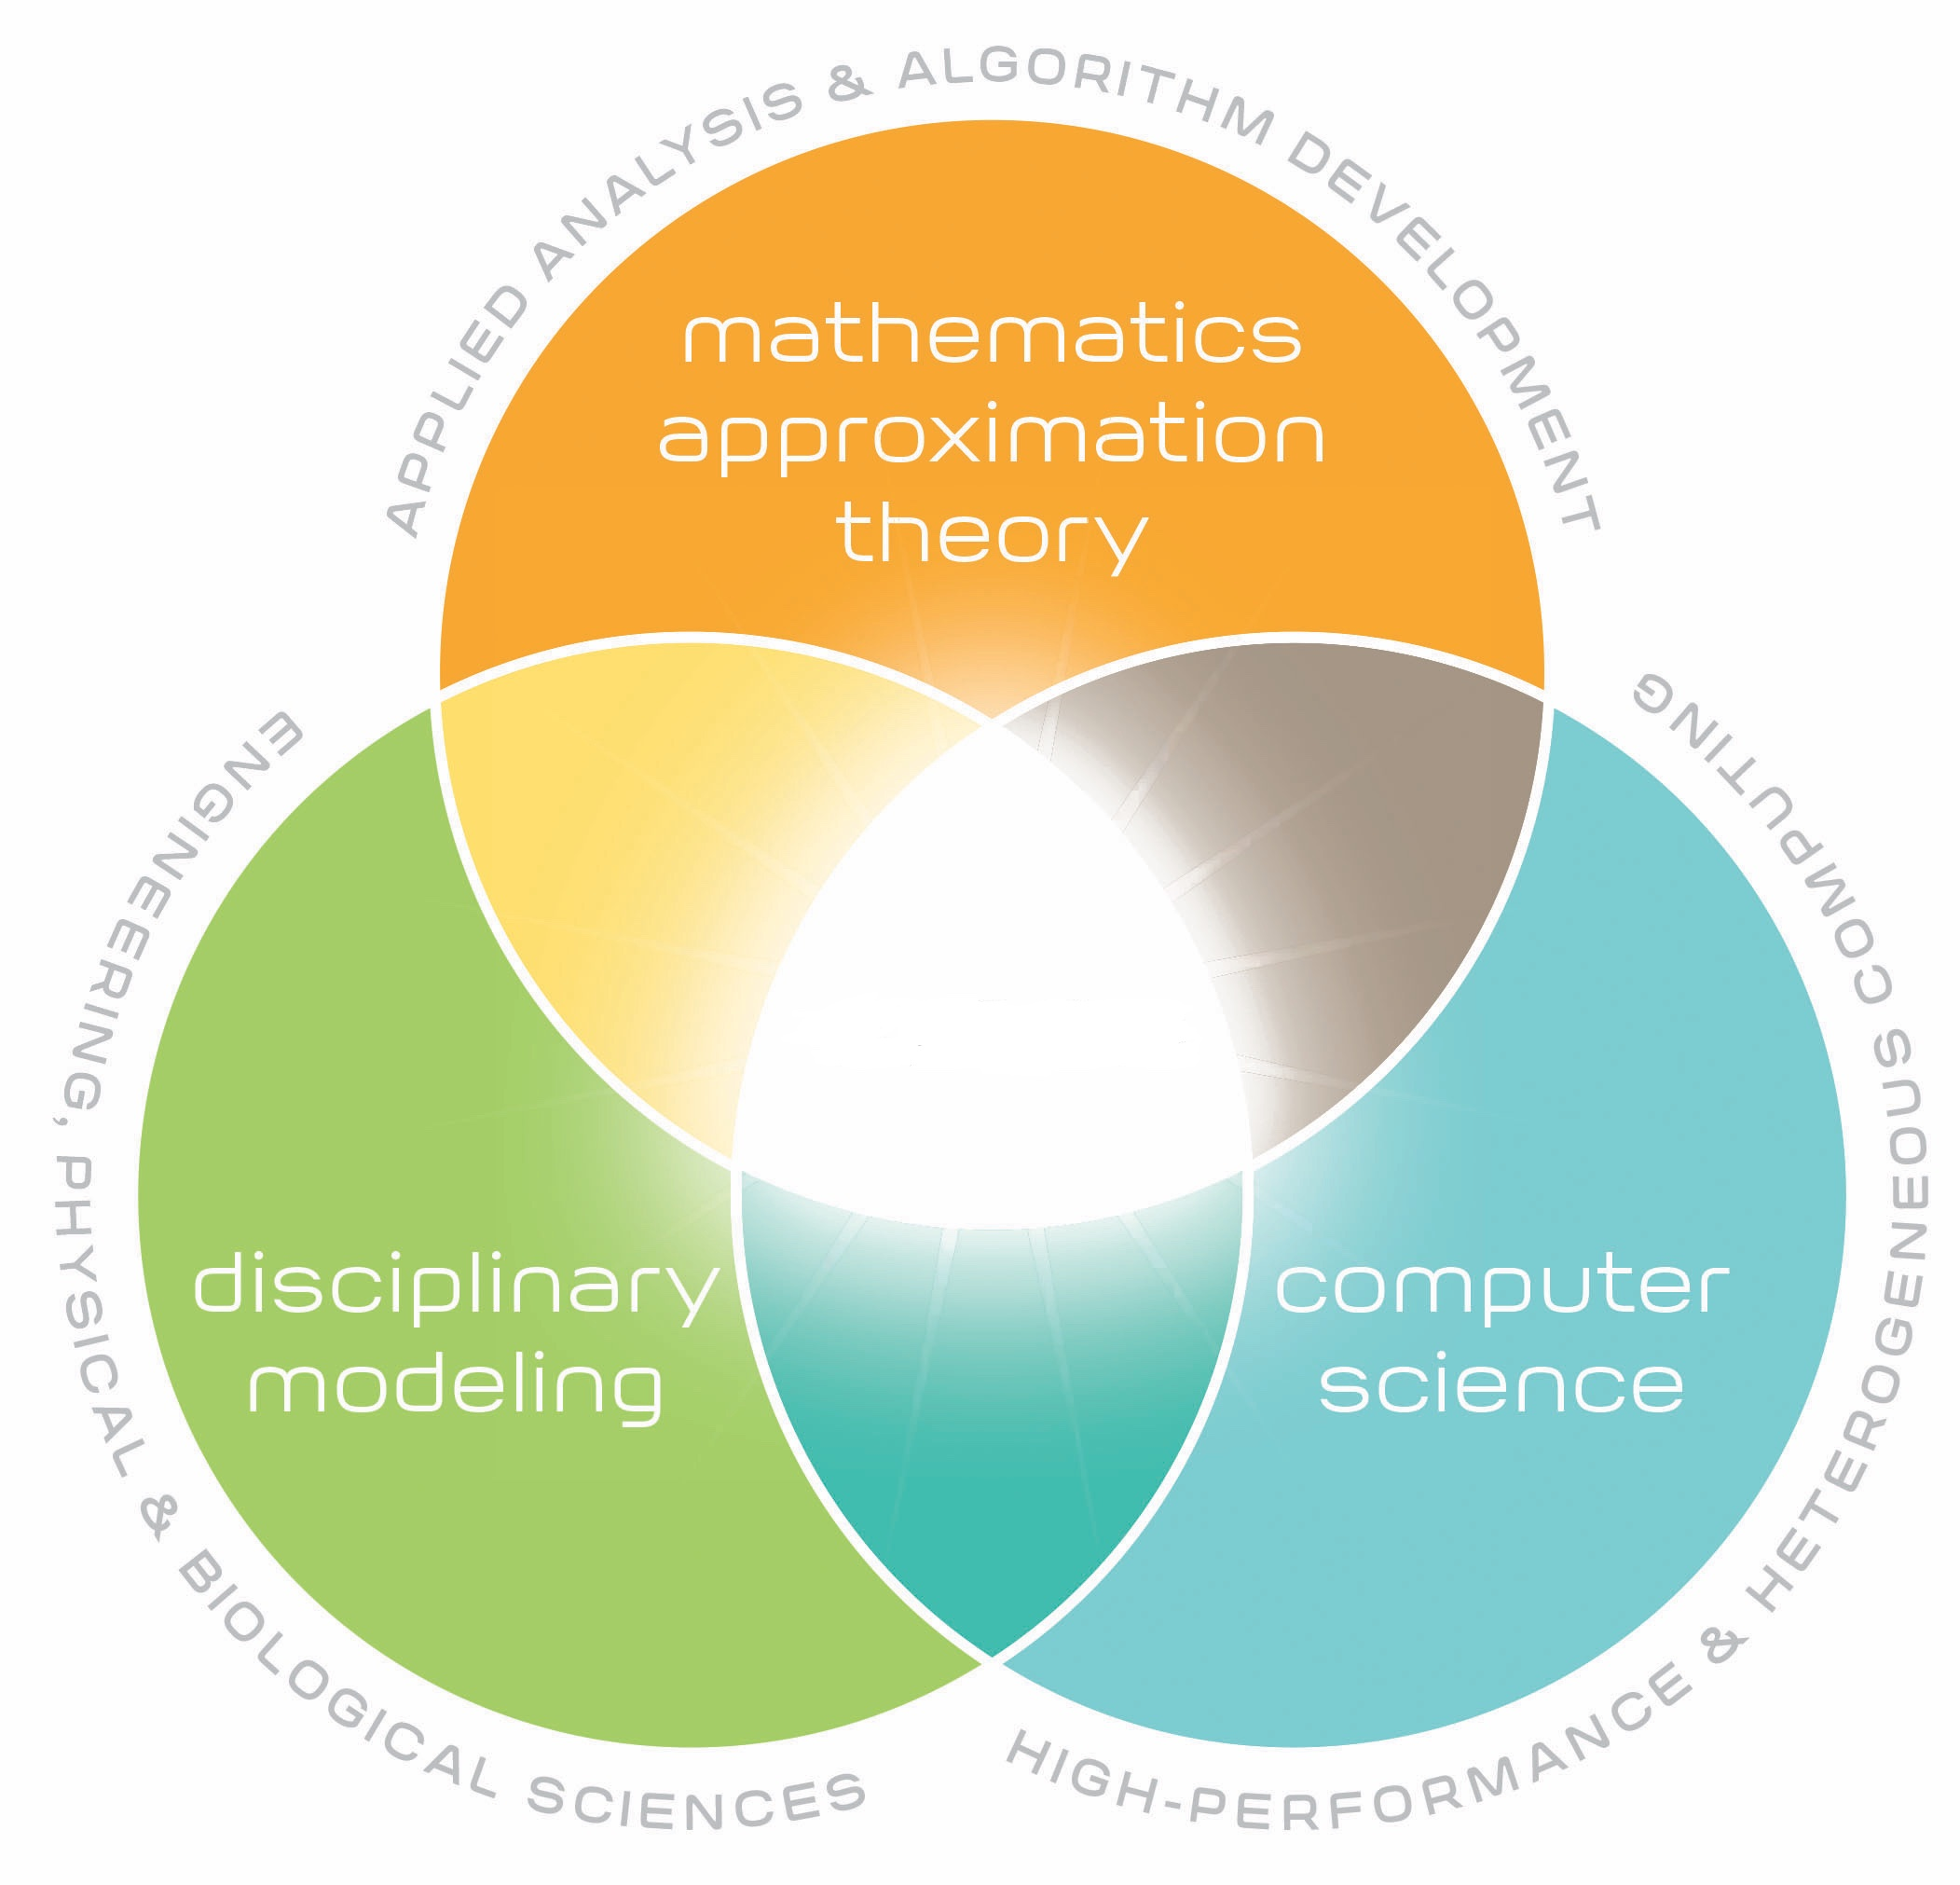
\includegraphics[width=0.6\linewidth]{figslides/cs.jpg}}

\vspace{6mm}

% !split
\subsection{Vision for the future: Scientific Computing and Data Science}

Scientific computing focuses on the development of predictive computer
models of the world around us. As study of physical phenomena through
experimentation has become impossible, impractical and/or expensive,
computational modeling has become the primary tool for
understanding—equal in stature to analysis and experiment. 
The discipline of scientific computing
is the development of new methods that make challenging problems
tractable on modern computing platforms, providing scientists and
engineers with key windows into the world around us.

Data science focuses on the development of tools designed to find
trends within datasets that help scientists who are challenged with
massive amounts of data to assess key relations within those
datasets. These key relations provide hooks that allow scientists to
identify models which, in turn, facilitate making accurate predictions
in complex systems. For example, a key data science goal on the
biological side would be better care for patients (e.g., personalized
medicine). Given a patient’s genetic makeup, the proper data-driven
model would identify the most effective treatment for that patient.

% !split
\subsection{Aims of the program}

A specific aim of this program is to develop the students' ability to pose and
solve problems that combine physical insights with mathematical tools
and computational skills. This provides a unique combination
of applied and theoretical knowledge and skills. These features are invaluable
for the development of multi-disciplinary educational and research programs.
The main focus is not to educate computer
specialists, but to educate students with a solid understanding in basic science
as well as an integrated knowledge on how  to use
essential methods from computational science. This requires an
education that covers both the specific disciplines like physics, biology,
geoscience, mathematics etc with a strong background in computational science.

A significant aspect of this program is the ability to offer new educational
opportunities that are aligned with the needs of a 21st century
workforce. Many companies are seeking
individuals who have knowledge of both a specific discipline and
computational modeling.

We plan to offer first Master of Science degrees in Computational Science
and  our students will be expressly educated in the use of
computing to model and study the world around them. Students in the CS
program will achieve a high degree of proficiency in model
development, critical thinking and analysis.

% !split
\subsection{Scientific and educational motivation}


% --- begin paragraph admon ---
\paragraph{Applications of simulation.}
Numerical simulations of various systems in science are central to our
basic understanding of nature and technlogy.
The increase in computational power,
improved algorithms for solving problems in science as well as access
to high-performance facilities, allow researchers nowadays to study
complicated systems across many length and energy scales. Applications
span from studying quantum physical systems in nanotechnology and the
characteristics of new materials or subamotic physics at its smallest
length scale, to simulating galaxies and the evolution of the universe.
In between, simulations are key to understanding
cancer treatment and how the brain works,
predicting climate changes and this week's weather,
simulating natural disasters, semi-conductor devices,
quantum computers, as well as assessing risk in the insurance and
financial industry. These are just a few topics
already well covered at the University of Oslo and that can be
topics for coming thesis projects as well as research directions.
% --- end paragraph admon ---




% --- begin paragraph admon ---
\paragraph{Job market.}
A large number of the candidates from the five involved departments
get jobs where numerical simulations are central and essential. The proposed
program will raise the educational quality in this area, because
our candidates need a broader understanding of the possibilities
and limitations of computation-based problem solving.
% --- end paragraph admon ---



% !split
\subsection{Multiscale modeling is a big open research question}


% --- begin paragraph admon ---
\paragraph{}
Today's problems, unlike traditional
science and engineering, involve complex systems with many distinct
physical processes. The wide open research topic of this century, both
in industry and at universities, is how to effectively couple
processes across different length and energy scales. Progress will
rely on a multi-disciplinary approach and therefore a need for
a multi-disciplinary educational program.
% --- end paragraph admon ---




% --- begin paragraph admon ---
\paragraph{}
The proposed program will foster candidates with the right
multi-disciplinary background and computational thinking for
understanding today's simulation technology and its challenges.
% --- end paragraph admon ---



% !split
\subsection{The new program combines old and new initiatives}

% --- begin paragraph admon ---
\paragraph{}

This program builds on the strengths and successes of two existing Master of Science directions at the University of Oslo, namely the 
programs in Computational Physics (at the Dept.~of Physics) and
Applied Mathematics and Mechanics (at the Dept.~of Mathematics).
These programs were established in 2003.
Based on the experience from these programs, the hope is that the proposed program can enlarge the reach of disciplines where computations play and/or are expected to play  a large. In particular, new directions 
in Computational Life Science need to  be developed to
meet coming needs of the scientific community. We believe this new direction is
best developed in close collaboration with already successful
computational science programs.
% --- end paragraph admon ---



% !split
\subsection{Computing competence}

% --- begin paragraph admon ---
\paragraph{}
Computing means solving scientific problems using computers. It covers
numerical as well as symbolic computing. Computing is also about
developing an understanding of the scientific process by enhancing
algorithmic thinking when solving problems.  Computing competence has
always been a central part of the science and engineering
education.

Modern computing competence is about

\begin{itemize}
\item derivation, verification, and implementation of algorithms

\item understanding what can go wrong with algorithms

\item overview of important, known algorithms

\item understanding how algorithms are used to solve mathematical problems

\item reproducible science and ethics

\item algorithmic thinking for gaining deeper insights about scientific problems
\end{itemize}

\noindent
% --- end paragraph admon ---



% !split
\subsection{Key elements in computing competence}

% --- begin paragraph admon ---
\paragraph{}
The power of the scientific method lies in identifying a given problem
as a special case of an abstract class of problems, identifying
general solution methods for this class of problems, and applying a
general method to the specific problem (applying means, in the case of
computing, calculations by pen and paper, symbolic computing, or
numerical computing by ready-made and/or self-written software). This
generic view on problems and methods is particularly important for
understanding how to apply available, generic software to solve a
particular problem.

Computing competence represents a central element
in scientific problem solving, from basic education and research to
essentially almost all advanced problems in modern
societies. Computing competence is simply central to further
progress. It enlarges the body of tools available to students and
scientists beyond classical tools and allows for a more generic
handling of problems. Focusing on algorithmic aspects results in
deeper insights about scientific problems.

Today's projects in science and industry tend to involve larger teams. Tools for reliable collaboration must therefore be mastered (e.g., version control systems, automated computer experiments for reproducibility, software and method documentation).
% --- end paragraph admon ---



% !split
\subsection{Overarching description of the CS program}

% --- begin paragraph admon ---
\paragraph{}
Students of this program learn to use the computer as a laboratory for
solving problems in science and engineering. The program offers
exciting thesis projects from many disciplines: biology and life
science, chemistry, mathematics, informatics, physics, geophysics,
mechanics, geology, computational finance, computational informatics, b
ig data analysis, digital signal processing
and image analysis – the candidates select research field according to
their interests.

A Master’s degree from this program gives the candidate a methodical
training in planning, conducting, and reporting large research
projects, often together with other students and university teachers.
THe projects emphasize finding practical solutions, developing an
intuitive understanding of the science and the scientific methods
needed to solve complicated problems, use of many tools, and not least
developing own creativity and independent thinking. The thesis
work is a scientific project where the candidates learn to tackle a
scientific problem in a professional manner.   The program aims also at
developing a deep understanding of the role of computing in solving modern scientific
problems. A candidate from this program gains  deep insights in the fundamnetal role
computations play  in our advancement of science and technology, as well as the role computations play  in society.
% --- end paragraph admon ---



% !split
\subsection{The program opens up for flexible backgrounds}


% --- begin paragraph admon ---
\paragraph{}
While discipline-based master's programs tend to introduce very strict
requirements to courses, we believe in adapting a computational thesis
topic to the student's background, thereby opening up for
students with a wide range of bachelor's degrees.
A very heterogeneous student community is thought to be a strength and
unique feature of this program.
% --- end paragraph admon ---



% !split
\subsection{Thesis directions}

% --- begin paragraph admon ---
\paragraph{}

\begin{itemize}
\item Computational Science: Applied Mathematics and Risk Analysis

\item Computational Science: Astrophysics

\item Computational Science: Bioinformatics

\item Computational Science: Biology

\item Computational Science: Chemistry

\item Computational Science: Geoscience

\item Computational Science: Imaging and Biomedical Computing

\item Computational Science: Materials science

\item Computational Science: Mechanics

\item Computational Science: Physics
\end{itemize}

\noindent
The thesis projects will be tailored to the student's needs, wishes and scientific background. The projects can easily incorporate topics from more than one discipline.
% --- end paragraph admon ---



% !split
\subsection{Structure and courses}

% --- begin paragraph admon ---
\paragraph{}
The table here is an example of a suggested path for a Master of Science project,
with course work the first year and thesis work the last year.


\begin{quote}
\begin{tabular}{llll}
\hline
\multicolumn{1}{l}{  } & \multicolumn{1}{l}{ 10 ECTS } & \multicolumn{1}{l}{ 10 ECTS } & \multicolumn{1}{l}{ 10 ECTS } \\
\hline
4th semester & Master thesis  & Master Thesis  & Master Thesis  \\
\hline
3rd semester & Master thesis  & Master Thesis  & Master Thesis  \\
\hline
2nd semester & Master courses & Master courses & Master courses \\
\hline
1st semester & Master courses & Master courses & Master courses \\
\hline
\end{tabular}
\end{quote}

\noindent
The program is very flexible in its structure and students may opt for starting with their thesis
work from the first semester and scatter the respective course load across all four semesters.
Depending on interests and specializations, there are many courses on computational science which can make
up the required curriculum of course work. Furthermore, courses may be broken up in smaller modules,
avoding thereby the limitation of 10 ECTS per course only. Some of these courses are listed below.
% --- end paragraph admon ---



% !split
\subsection{Presently available courses at UiO and NMBU}

% --- begin paragraph admon ---
\paragraph{}

\begin{itemize}
\item \href{{http://www.uio.no/studier/emner/matnat/fys/FYS4150/index-eng.html}}{FYS4150 Computational Physics I}

\item \href{{http://www.uio.no/studier/emner/matnat/fys/FYS4411/}}{FYS4411 Computational Physics II}

\item \href{{http://www.uio.no/studier/emner/matnat/fys/FYS4460/}}{FYS4460 Computational Physics III}

\item \href{{http://www.uio.no/studier/emner/matnat/ifi/INF5620/index-eng.html}}{INF5620 Numerical Methods for Partial Differential Equations}

\item \href{{http://www.uio.no/studier/emner/matnat/ifi/INF5631/index-eng.html}}{INF5631 Project on Numerical Methods for Partial Differential Equations}

\item \href{{http://www.nmbu.no/course/FYS388}}{FYS388 Computational Neuroscience}

\item \href{{http://www.uio.no/studier/emner/matnat/math/STK4520/index-eng.html}}{STK4520 Laboratory for Finance and Insurance Mathematics}

\item \href{{http://www.uio.no/studier/emner/matnat/math/STK4021/index-eng.html}}{STK4021 Applied Bayesian Analysis and Numerical Methods}

\item \href{{http://www.uio.no/studier/emner/matnat/math/MAT-INF4130/index-eng.html}}{MAT-INF4130  Numerical Linear Algebra}

\item \href{{http://www.uio.no/studier/emner/matnat/math/MAT-INF4110/index.html}}{MAT-INF4110 Mathematical Optimization}

\item \href{{http://www.uio.no/studier/emner/sv/oekonomi/ECON4240/index.html}}{ECON4240 Equilibrium, welfare and information}

\item \href{{http://www.uio.no/studier/emner/matnat/math/MEK4470/index-eng.html}}{MEK4470  Computational Fluid Mechanics}

\item \href{{http://www.uio.no/studier/emner/matnat/math/MEK4250/index-eng.html}}{MEK4250 Finite Element Methods in Computational Mechanics}

\item \href{{http://www.uio.no/studier/emner/matnat/geofag/GEO4310/}}{GEO4310 - Stochastic methods in hydrology}

\item \href{{http://www.uio.no/studier/emner/matnat/astro/AST5210/index-eng.html}}{AST5210 Stellar Atmospheres I}

\item \href{{http://www.uio.no/studier/emner/matnat/astro/AST9110/index-eng.html}}{AST9110 Numerical Modeling}
\end{itemize}

\noindent
% --- end paragraph admon ---



% !split
\subsection{New courses}

% --- begin paragraph admon ---
\paragraph{}
In order to build a common study program and identity as a Computational Science student, there will be two compulsory courses that aim at providing topics of common and broad interest.
Both courses have a workload of 10 ECTS each. The courses are

\begin{itemize}
\item \textbf{CS-MATH1}: \emph{Data analysis and machine learning}, 10 ECTS (Existing \href{{http://www.uio.no/studier/emner/matnat/math/STK2100/}}{STK2100}, \href{{http://www.uio.no/studier/emner/matnat/geofag/GEO4310/}}{GEO4310})
\begin{enumerate}

 \item Monte Carlo methods and statistical data analysis

 \item Optimization of data and handling of large data sets

 \item Machine learning and neural networks

\end{enumerate}

\noindent
\item \textbf{CS-INF1}: \emph{High-Performance Computing and Numerical projects}, 10 ECTS (Existing INF3380)
\begin{enumerate}

 \item This course teaches you to develop and structure large numerical projects, from code writing to  finalizing a report

 \item Topics which are included are parallelization and vectorization

 \item Machine architecture and GPU-CPU programming

 \item Optimization of code and benchmarking

 \item Numerical methods from linear algebra will be discussed as well as examples from life science.
\end{enumerate}

\noindent
\end{itemize}

\noindent
% --- end paragraph admon ---



% !split
\subsection{Possible new courses}
Some of these courses could incorporate (or base themselves upon) existing ones. The courses here are organized according to their corresponding disciplines. They should, for search ease, contain the word \textbf{Computational} 
\begin{itemize}
\item Mathematics
\begin{enumerate}

\item \textbf{CS-MATH1}: Data analysis and machine learning (Existing \href{{http://www.uio.no/studier/emner/matnat/geofag/GEO4330/}}{GEO4330}, STK2100)

\item \textbf{CS-MATH2}: Basic methods in computational modeling   (new? do we need it?)

\item \textbf{CS-MATH3}: Mathematical Foundations of data science (based on MAT-INF4110 and STK4021)

\item \textbf{CS-MATH4}: Computational Linear Algebra (based on MAT-INF4130)

\item \textbf{CS-MATH5}: Computational differential equations (Based on INF5620)

\item \textbf{CS-MATH6}: Computational finance (based on STK4520)

\item \textbf{CS-MATH7}: Advanced data science (new)

\end{enumerate}

\noindent
\item Physical sciences (Astrophysics, geoscience, physics, chemistry and materials science)
\begin{enumerate}

\item \textbf{CS-PHYS1}: Computational Physics (based on FYS3150/4150)

\item \textbf{CS-PHYS2}: Computational Molecular dynamics in life science and materials science (new)

\item \textbf{CS-PHYS3}: Computational Astrophysics (based on AST9110)

\item \textbf{CS-PHYS4}: Computational quantum mechanics (based on fys4411 and FYS-MENA4110)

\item \textbf{CS-PHYS5}: Computational statistical mechanics (based on fys4460)

\item \textbf{CS-PHYS6}: Computational Materials Science (based on FYS-MENA4111)

\end{enumerate}

\noindent
\item Bioscience
\begin{enumerate}

\item \textbf{CS-BIO1}: Computational Bioinformatics (Based on INF5380)

\item \textbf{CS-BIO2}: Advanced Computational bioinformatics (new)

\item \textbf{CS-PHYS2}: Computational Molecular dynamics in life science and materials science (new)

\end{enumerate}

\noindent
\item Computer science
\begin{enumerate}

\item \textbf{CS-INF1}: High-Performance Computing and Numerical projects (parts of inf3380, else new)

\item \textbf{CS-INF2}: Advanced optimization of numerical code (new)

\end{enumerate}

\noindent
\item Mechanics
\begin{enumerate}

\item \textbf{CS-MECH1}: Computational Mechanics (based on MEK4470 and MEK4250?)

\item \textbf{CS-MECH2}: Advanced Computational Mechanics (new?)
\end{enumerate}

\noindent
\end{itemize}

\noindent
% !split
\subsection{Graduate Certificates}
The program plans to offer graduate certificates in
\begin{itemize}
\item Three of the courses with label CS-MATH  gives a certificate in Computational Mathematics

\item Three of the courses with label CS-PHYS gives a certificate in Computational Physics, Astrophysics, Chemistry, Materials Science  and Geoscience

\item Three of the courses with label CS-BIO gives a certificate in Computational life science. 

\item Three of the courses with label CS-INF gives a certificate in High-performance computing. 
\end{itemize}

\noindent
% !split 
\subsection{Description of Study directions}

The basic structure of the study directions could be

\begin{itemize}
\item Description of study directions with potential projects

\item Admission criteria

\item Learning outcomes

\item Program structure

\item Semester abroad

\item Career prospects

\item Teaching and examinations
\end{itemize}

\noindent
What follows are text proposals for these items.

% !split
\subsection{Admission criteria: Applied Mathematics and Risk Analysis}

This study direction requires 90 ECTS in mathematics and informatics courses. 
\begin{enumerate}
\item 70 ECTS have to be from the following courses, equivalent or similar to the University of Oslo mathematics and programming courses MAT1110, MAT1120, MAT2100/MAT2400, STK1100, MAT-INF1100, INF1000/INF1110 and IN2900 (new code). 

\item In addition, 20 ECTS have to come from at least  two of the advanced courses MAT-INF3100, MAT-INF3360, STK2130, STK3405, INF3311, MAT-INF3xxx (Numerical analysis, new code) and/or MAT-INF3yyy (Dynamical systems, new code).

\item An average mark C (European grading scale) is required for the above courses.
\end{enumerate}

\noindent
% !split
\subsection{Admission criteria: Astrophysics}
The program has a minimum course requirement of 120 ECTS (European Credit Transfer System) at the undergraduate level (bachelor degree or equivalent) in astrophysics, bioscience, chemistry, computer science and informatics, geoscience, mathematics, materials science, mechanics and physics. 
\begin{enumerate}
\item Of these 120 ECTS, 40 ECTS have to include basic mathematics and programming courses, equivalent to the University of Oslo mathematics courses MAT1100, MAT1110, MAT1120 and at least one of the corresponding computing and programming courses INF1000/INF1110 or MAT-INF1100/MAT-INF1100L/BIOS1100/KJM-INF1xxx. 

\item The remaining 80 ECTS have to be within at most two of the fields of astrophysics, bioscience, chemistry, computer science and informatics, geoscience, mathematics, materials science, mechanics and physics. 40 of these 80 ECTS have to be advanced undergraduate courses at the 2000 and 3000 level and a minimum of 20 ECTS must be at the 3000 level within physics/material science/astrophysics/informatics/mathematics/mechanics. 

\item An average mark C (European grading scale) is required for the 40 ECTS in mathematics and programming (corresponding  to the University of Oslo courses  MAT1100, MAT1110, MAT1120  and the corresponding computing and programming courses INF1000/INF1110 or MAT-INF1100/MAT-INF1100L/BIOS1100/KJM-INF1xxx or similar courses) and the 40 ECTS at the 2000 and 3000 level. A minimum of 20 ECTS must be at the 3000 level within physics/material science/astrophysics/informatics/mathematics/mechanics. 
\end{enumerate}

\noindent
% !split
\subsection{Admission criteria: Bioinformatics}

The program has a minimum course requirement of 120 ECTS (European Credit Transfer System) at the undergraduate level (bachelor degree or equivalent) in Astrophysics, bioscience, chemistry, computer science and informatics, geoscience, mathematics, materials science, mechanics and physics. 
\begin{enumerate}
\item Of these 120 ECTS, 80 ECTS have to be within Informatics/Mathematics/Statistics (courses labeled as INF/IN, INF-MAT, MAT-INF, MAT and STK) where of 50 ECTS have to include basic mathematics and programming courses, equivalent to the University of Oslo mathematics courses MAT1100, MAT1110, MAT1120 and the corresponding computing and programming courses INF1000/INF1110 and INF1010/IN2900. 

\item A total of at least 40 ECTC out of the 120 ECTC have to be advanced undergraduate courses at the 2000 and 3000 level.

\item An average mark C (European grading scale) is required for the above-specified 80 ECTS in Informatics/Mathematics/Statistics.
\end{enumerate}

\noindent
% !split
\subsection{Admission criteria: Bioscience}

The program has a minimum course requirement of 120 ECTS (European Credit Transfer System) at the undergraduate level (bachelor degree or equivalent) in Astrophysics, bioscience, chemistry, computer science and informatics, geoscience, mathematics, materials science, mechanics and physics. 
\begin{enumerate}
\item Of these 120 ECTS, 40 ECTS have to include basic mathematics and programming courses, equivalent to the University of Oslo mathematics courses MAT1100, MAT1110, MAT1120 and at least one of the corresponding computing and programming courses INF1000/INF1110 or MAT-INF1100/MAT-INF1100L/BIOS1100/KJM-INF1xxx. 

\item The remaining 80 ECTS have to be within at most two of the fields of astrophysics, bioscience, chemistry, computer science and informatics, geoscience, mathematics, materials science, mechanics and physics. 40 of these 80 ECTS have to be advanced undergraduate courses at the 2000 and 3000 level and a minimum of 20 ECTS must be at the 3000 level within bioscience. 

\item An average mark C (European grading scale) is required for the 40 ECTS in mathematics and programming (corresponding  to the University of Oslo courses  MAT1100, MAT1110, MAT1120  and the corresponding computing and programming courses INF1000/INF1110 or MAT-INF1100/MAT-INF1100L/BIOS1100/KJM-INF1xxx or similar courses) and the 40 ECTS at the 2000 and 3000 level. A minimum of 20 ECTS must be at the 3000 level within bioscience.
\end{enumerate}

\noindent
% !split
\subsection{Admission criteria: Chemistry}

The program has a minimum course requirement of 120 ECTS (European Credit Transfer System) at the undergraduate level (bachelor degree or equivalent) in Astrophysics, bioscience, chemistry, computer science and informatics, geoscience, mathematics, materials science, mechanics and physics. 
\begin{enumerate}
\item Of these 120 ECTS, 40 ECTS have to include basic mathematics and programming courses, equivalent to the University of Oslo mathematics courses MAT1100, MAT1110, MAT1120, MAT1050 and MAT1060 and at least one of the corresponding computing and programming courses INF1000/INF1110 or MAT-INF1100/MAT-INF1100L/BIOS1100/KJM-INF1xxx/GEO-KJM1040. 

\item The remaining 80 ECTS have to be within at most two of the fields of astrophysics, bioscience, chemistry, computer science and informatics, geoscience, mathematics, materials science, mechanics and physics. 40 of these 80 ECTS have to be advanced undergraduate courses at the 2000 and 3000 level and a minimum of 20 ECTS must be at the 3000 level within physics/material science/mechanics/astrophysics/informatics/mathematics/bioscience/chemistry/geoscience.

\item An average mark C (European grading scale) is required for the 40 ECTS in mathematics and programming (corresponding  to the University of Oslo courses  MAT1100, MAT1110, MAT1120, MAT1050 and MAT1060  and the corresponding computing and programming courses INF1000/INF1110 or MAT-INF1100/MAT-INF1100L/BIOS1100/KJM-INF1xxx/GEO-KJM1040 or similar courses) and the 40 ECTS at the 2000 and 3000 level. A minimum of 20 ECTS must be at the 3000 level within physics/material science/astrophysics/mechanics/mathematics/informatics/bioscience/chemistry/geoscience.
\end{enumerate}

\noindent
% !split
\subsection{Admission criteria: Geoscience}

The program has a minimum course requirement of 120 ECTS (European Credit Transfer System) at the undergraduate level (bachelor degree or equivalent) in Astrophysics, bioscience, chemistry, computer science and informatics, geoscience, mathematics, materials science, mechanics and physics. 
\begin{enumerate}
\item Of these 120 ECTS, 40 ECTS have to include basic mathematics and programming courses, equivalent to the University of Oslo mathematics courses MAT1100, MAT1110, MAT1120  and at lest one of the corresponding computing and programming courses INF1000/INF1110 or MAT-INF1100/MAT-INF1100L/BIOS1100/GEO1040/GEO-KJM1040. 

\item The remaining 80 ECTS have to be within at most two of the fields of astrophysics, bioscience, chemistry, computer science and informatics, geoscience, mathematics, materials science, mechanics and physics. 40 of these 80 ECTS have to be advanced undergraduate courses at the 2000 and 3000 level in the fields of astrophysics, bioscience, chemistry, computer science and informatics, geoscience, mathematics, materials science, mechanics and physics.

\item An average mark C (European grading scale) is required for the 40 ECTS in mathematics and programming (corresponding  to the University of Oslo courses  MAT1100, MAT1110, MAT1120  and the corresponding computing and programming courses INF1000/INF1110 or MAT-INF1100/MAT-INF1100L/BIOS1100/GEO1040/GEO-KJM1040 or similar courses) and the 40 ECTS at the 2000 and 3000 level within the fields of astrophysics, bioscience, chemistry, computer science and informatics, geoscience, mathematics, materials science, mechanics and physics.
\end{enumerate}

\noindent
% !split
\subsection{Admission criteria: Imaging and Biomedical Computing}

The program has a minimum course requirement of 120 ECTS (European Credit Transfer System) at the undergraduate level (bachelor degree or equivalent) in Astrophysics, bioscience, chemistry, computer science and informatics, geoscience, mathematics, materials science, mechanics and physics. 
\begin{enumerate}
\item Of these 120 ECTS, 80 ECTS have to be within Informatics/Mathematics/Statistics (courses labeled as INF/IN, INF-MAT, MAT-INF, MAT and STK) where of 50 ECTS have to include basic mathematics and programming courses, equivalent to the University of Oslo mathematics courses MAT1100, MAT1110, MAT1120 and the corresponding computing and programming courses INF1000/INF1110 and INF1010/IN2900. 

\item A total of at least 40 ECTC out of the 120 ECTC have to be advanced undergraduate courses at the 2000 and 3000 level.

\item An average mark C (European grading scale) is required for the above-specified 80 ECTS in Informatics/Mathematics/Statistics.
\end{enumerate}

\noindent
% !split
\subsection{Admission criteria: Materials Science}

The program has a minimum course requirement of 120 ECTS (European Credit Transfer System) at the undergraduate level (bachelor degree or equivalent) in Astrophysics, bioscience, chemistry, computer science and informatics, geoscience, mathematics, materials science, mechanics and physics. 
\begin{enumerate}
\item Of these 120 ECTS, 40 ECTS have to include basic mathematics and programming courses, equivalent to the University of Oslo mathematics courses MAT1100, MAT1110, MAT1120 and at least one of the corresponding computing and programming courses INF1000/INF1110 or MAT-INF1100/MAT-INF1100L/BIOS1100/KJM-INF1xxx. 

\item The remaining 80 ECTS have to be within at most two of the fields of astrophysics, bioscience, chemistry, computer science and informatics, geoscience, mathematics, materials science, mechanics and physics. 40 of these 80 ECTS have to be advanced undergraduate courses at the 2000 and 3000 level and a minimum of 20 ECTS must be at the 3000 level within physics/material science/astrophysics/informatics/mathematics/bioscience/chemistry/mechanics/geoscience.

\item An average mark C (European grading scale) is required for the 40 ECTS in mathematics and programming (corresponding  to the University of Oslo courses  MAT1100, MAT1110, MAT1120  and the corresponding computing and programming courses INF1000/INF1110 or MAT-INF1100/MAT-INF1100L/BIOS1100/KJM-INF1xxx or similar courses) and the 40 ECTS at the 2000 and 3000 level. A minimum of 20 ECTS must be at the 3000 level within physics/material science/astrophysics/mathematics/mechanics/informatics/bioscience/chemistry/geoscience.
\end{enumerate}

\noindent
% !split 
\subsection{Admission Criteria: Mechanics}

\begin{enumerate}
\item The program requires 80 ECTS within the  basic mathematics and programming courses, equivalent to the University of Oslo mathematics courses MAT1100, MAT1110, MAT1120, MEK1100, MEK2200, INF1000/INF1100, MAT-INF3360.

\item In addition, the program requires  one of the following courses INF3331, MAT-INF3100, MAT-INF3xxx (Numerical analysis, new code) and/or MAT-INF3yyy (Dynamical systems, new code). 

\item An average mark C (European grading scale) is required for these courses.
\end{enumerate}

\noindent
% !split 
\subsection{Admission Criteria: Physics}
The program has a minimum course requirement of 120 ECTS (European Credit Transfer System) at the undergraduate level (bachelor degree or equivalent) in Astrophysics, bioscience, chemistry, computer science and informatics, geoscience, mathematics, materials science, mechanics and physics. 
\begin{enumerate}
\item Of these 120 ECTS, 40 ECTS have to include basic mathematics and programming courses, equivalent to the University of Oslo mathematics courses MAT1100, MAT1110, MAT1120 and at least one of the corresponding computing and programming courses INF1000/INF1110 or MAT-INF1100/MAT-INF1100L/BIOS1100/KJM-INF1xxx. 

\item The remaining 80 ECTS have to be within at most two of the fields of astrophysics, bioscience, chemistry, computer science and informatics, geoscience, mathematics, materials science, mechanics and physics. 40 of these 80 ECTS have to be advanced undergraduate courses at the 2000 and 3000 level and a minimum of 20 ECTS must be at the 3000 level within physics/material science/mechanics/astrophysics/informatics/mathematics/bioscience/chemistry/geoscience.

\item An average mark C (European grading scale) is required for the 40 ECTS in mathematics and programming (corresponding  to the University of Oslo courses  MAT1100, MAT1110, MAT1120  and the corresponding computing and programming courses INF1000/INF1110 or MAT-INF1100/MAT-INF1100L/BIOS1100/KJM-INF1xxx or similar courses) and the 40 ECTS at the 2000 and 3000 level. A minimum of 20 ECTS must be at the 3000 level within physics/material science/astrophysics/mechanics/mathematics/informatics/bioscience/chemistry/geoscience.
\end{enumerate}

\noindent
% !split
\subsection{Description of learning outcomes}

The power of the scientific method lies in identifying a given problem
as a special case of an abstract class of problems, identifying
general solution methods for this class of problems, and applying a
general method to the specific problem (applying means, in the case of
computing, calculations by pen and paper, symbolic computing, or
numerical computing by ready-made and/or self-written software). This
generic view on problems and methods is particularly important for
understanding how to apply available, generic software to solve a
particular problem.

Computing competence represents a central element
in scientific problem solving, from basic education and research to
essentially almost all advanced problems in modern
societies. Computing competence is simply central to further
progress. It enlarges the body of tools available to students and
scientists beyond classical tools and allows for a more generic
handling of problems. Focusing on algorithmic aspects results in
deeper insights about scientific problems.

The learning outcomes are subdivided in three general categories, knowledge, skills and general competence.

\begin{itemize}
\item \textbf{Knowledge}: A candidate from this program
\begin{itemize}

 \item has deep knowledge of the scientific method and computational science at an advanced level, meaning that the candidate
\begin{enumerate}

 \item has the ability to understand advanced scientific results in new fields

 \item has fundamental understanding of methods and tools

 \item can develop and apply advanced computational methods to scientific problems

 \item is capable of judging and analyzing all parts of the obtained scientific results

 \item can present results orally and in written form as scientific reports/articles

 \item can propose new hypotheses and suggest solution paths

 \item can generalize mathematical algorithms and apply them to new situations

 \item can link computational models to specific applications and/or experimental data

 \item can develop models and algorithms to describe experimental data

\item masters methods for reproducibility and how to link this to a sound ethical scienfitic conduct

\item has a thorough understanding of how computing is used to  solve  scientific problems

\item knows fundamental algorithms in computational science

\end{enumerate}

\noindent
 \item has a fundamental understanding and knowledge of scientific work, meaning that
\begin{enumerate}

 \item the candidate can develop hypotheses and suggest ways to test these

 \item can use relevant analytical, experimental and numerical tools and results to test the scientific hypotheses

 \item can generalize from numerical and experimental data to mathematical models and underlying principles

 \item can analyze the results and evaluate their relevance with respect to the actual problems and/or hypotheses

 \item can present the results according to good scientific practices

\end{enumerate}

\noindent
\end{itemize}

\noindent
\item \textbf{Skills}: A candidate from this program
\begin{itemize}

 \item has a deep understanding of what computing means, entailing several or all of the topics listed below
\begin{enumerate}

 \item knows the most fundamental algorithms involved, how to optimize these and perform statistical uncertainty quantification

 \item has overview of advanced algorithms and how they can be accessed in available software and how they are used to solve scientific problems

 \item has knowledge and understands high-performance computing elements: memory usage, vectorization and parallel algorithms

 \item can use effeciently high-performance computing resources, from compilers to hardware architectures

 \item understands approximation errors and what can go wrong with algorithms

 \item has knowledge of at least one computer algebra system and how it is applied to perform classical mathematics

 \item has extensive experience with programming in a high-level language (MATLAB, Python, R)

 \item has experience with programming in a compiled language (Fortran, C, C++)

 \item has experience with implementing and applying numerical algorithms in reusable software that acknowledges the generic nature of the mathematical algorithms

\item has experience with debugging software

\item has experience with test frameworks and procedures

\item has experience with different visualization techniques for different types of data

\item can critically evaluate results and errors

\item can develop algorithms and software for complicated scientific problems independently and in collaboration with other students

\item masters software carpentry: can design a maintainable program in a systematic way, use version control systems, and write scripts to automate manual work

\item understands how to increase the efficiency of numerical algorithms and pertinent software

\item has knowledge of stringent requirements to efficiency and precision of software

\item understands tools to make science reproducible and has a sound ethical approach to scientific problems

\end{enumerate}

\noindent
\end{itemize}

\noindent
\item \textbf{General competence}: A candidate from this program
\begin{itemize}

 \item is able to develop professional competence through the thesis work, entailing:
\begin{enumerate}

 \item mature professionally and be able to work independently

 \item can communicate in a professional way scientific results, orally and in written form

 \item can plan and complete a research project

 \item can develop a scientific intuition and understanding that makes it possible to present and discuss scientific problems, results and uncertainties

\end{enumerate}

\noindent
 \item is able to develop virtues, values and attitudes that lead to  a better understanding of ethical aspects of the scientific method, as well as promoting central aspects of the scientific method to society. This means for example that the candidate
\begin{enumerate}

 \item can reflect on and develop strategies for making science reproducible and to promote the need for a proper ethical conduct

 \item has a deep understanding of the role basic and applied  research and computing play for progress in society

 \item is able to promote, use and develop version control tools in order to make science reproducible

 \item is able to critically evaluate the consequences of own research and how this impacts society

 \item matures an understanding of the links between basic and applied research and how these shape, in a fundamental way,  progress in science and technology

 \item can develop an understading of the role research and science can play together with industry and society in general

 \item can reflect over and develop learning strategies for life-long learning.
\end{enumerate}

\noindent
\end{itemize}

\noindent
\end{itemize}

\noindent
By completing a Master of Science thesis, the candidate will have developed a critical understanding of the scientific methods which have been studied, has a better understanding of the scientific process per se as well as having developed perspectives for future work and how to verify and validate scientific results.

% !split
\subsection{Study abroad and international collaborators}


% --- begin paragraph admon ---
\paragraph{}

Students at the University of Oslo may choose to take parts of
their degrees at a university abroad.

Students in this program have a number of interesting international
exchange possibilities. The involved researchers have extensive
collaborations with other researchers worldwide. These exchange
possibility range from top universities in the USA, Asia and Europe as
well as leading National Laboratories in the USA.
% --- end paragraph admon ---



% !split
\subsection{Career prospects}


% --- begin paragraph admon ---
\paragraph{}
Candidates who are capable of modeling and understanding complicated
systems in natural science, are in short supply in society.  The
computational methods and approaches to scientific problems students learn
when working on their thesis projects are very similar to the methods
they will use in later stages of their careers.  To handle large
numerical projects demands structured thinking and good analytical
skills and a thorough understanding of the problems to be solved. This
knowledge makes the students unique on the labor market.

Career opportunities are many, from research institutes, universities
and university colleges and a multitude of companies. Examples
include IBM, Hydro, Statoil, and Telenor.  The program gives an
excellent background for further studies, with a PhD as one possible
goal.

The program has also a strong international element which allows students to
gain important experience from international collaborations in
science, with the opportunity to spend parts of the time spent on
thesis work at research institutions abroad.
% --- end paragraph admon ---




% ------------------- end of main content ---------------

% #ifdef PREAMBLE
\end{document}
% #endif

